\ylDisplay{Jalgrattur} % Ülesande nimi
{Jaan Kalda} % Autor
{lõppvoor} % Voor
{2013} % Aasta
{G 3} % Ülesande nr.
{4} % Raskustase
{
% Teema: Kinemaatika
\ifStatement
Poiss mõõdab jalgrattaga sõites tuule kiirust enda suhtes: kui ta sõidab piki teed ühes
suunas kiirusega \SI{10}{km/h}, saab ta tulemuseks \SI{20}{km/h}, ning kui ta sõidab
vastassuunas kiirusega \SI{20}{km/h}, siis saab ta tulemuseks samuti
\SI{20}{km/h}. Kui kiiresti maa suhtes puhub tuul?
\fi


\ifHint
Vaadeldes tuule ja jalgratturi kiirusi vektoritena, on võimalik geomeetriliselt konstrueerida vastavad tekstis toodud tingimused ning geomeetria põhjal tuule kiirus välja arvutada.
\fi


\ifSolution
Jalgratturi mõõdetav tuul $\vec w'$ on tuule kiirusvektori $\vec w$ ja jalgratturi kiirusvektori $\vec v$ vahe $\vec w'=\vec w - \vec v$. Olgu jalgratturi kiirusvektorid $\vec v_1$ ja $\vec v_2$ ning tuule kiirusvektorid  $\vec w'_1$ ja $\vec w'_2$ vastavalt ühele ja teisele poole sõites.

Antud juhul teame ainult kiirusi, mitte nende suundi. Teades eelnevalt, et mõõdetud tuule kiirus on sama suur mõlemas suunas liikudes, saab kiirusvektorid esitada võrdhaarse kolmnurgana. (Kolmnurga mõlemad pooled vastavad erinevas suunas sõitmisele ning vastavad ülal mainitud valemile. Kuna tuule vektor on mõlemal juhul sama ja kiirused paralleelsed, saab selle konstrueerida nagu joonisel.)

\begin{center}
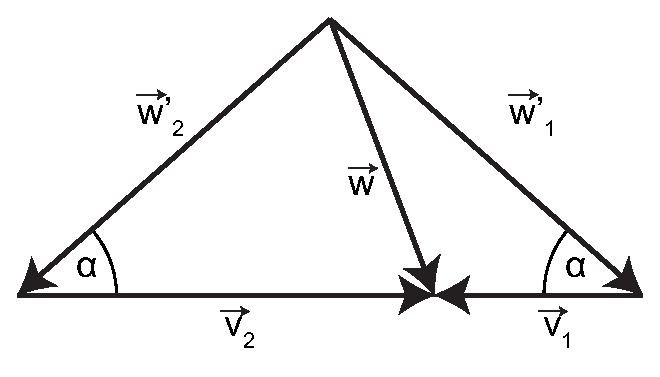
\includegraphics[width=0.4\textwidth]{2013-v3g-03-jalgrattur}\\
\end{center}

Koosinusteoreemist: 

$$
\begin{cases}
|\vec w|^2 = |\vec w'_1|^2 + |\vec v_1|^2  - 2  |\vec w'_2|  |\vec v_1|\cos \alpha \\
|\vec w|^2 = |\vec w'_2|^2 + |\vec v_2|^2  - 2  |\vec w'_2|  |\vec v_2|\cos \alpha.
\end{cases}
$$
Teades, et $ |\vec v_2|=2 |\vec v_1|$ ja et  $ |\vec w'_1|=2 |\vec w'_2|$, saame esimese võrrandi korrutada kahega ja teise sellest lahutada.

$$|\vec w|^2 = |\vec w'_1|^2 - 2|\vec v_1|^2. $$

Ehk  tuule tegelik kiirus on:
$$|\vec w|=\sqrt{|\vec w'_1|^2-2|\vec v_1|^2} \approx \SI{14}{km \per h}.$$
\fi


\ifEngStatement
% Problem name: Cyclist
A boy is measuring the speed of wind with respect to himself while riding on a bicycle: if he is riding along the road at one direction with a speed 10 km/h then he gets the result 20 km/h and if he rides the opposite direction with a speed 20 km/h then he also gets the result 20 km/h. How fast with respect to the ground is the wind blowing?
\fi


\ifEngHint
Observing the velocities of wind and the cyclist as vectors it is possible to geometrically construct the respective conditions given in the text and calculate the wind speed on the basis of geometry.
\fi


\ifEngSolution
The wind $\vec w'$ measured by the cyclist is the difference of wind’s velocity $\vec w$ and the cyclist’s velocity $\vec v$: $\vec w'=\vec w - \vec v$. Let the velocities of the cyclist be $\vec v_1$ and $\vec v_2$ and the velocities of the wind $\vec w'_1$ and $\vec w'_2$ respectively when driving along one direction and the other.\\
In the given case we only know the speeds and not their directions. Knowing from before that the measured speed of the wind is equal at both directions we can present the velocities as an isosceles triangle. (Both of the triangle’s sides correspond to cycling along either direction and meet the equation given above. Since the wind’s vector is the same for both cases and the velocities are parallel then we can construct as in the figure).
\begin{center}
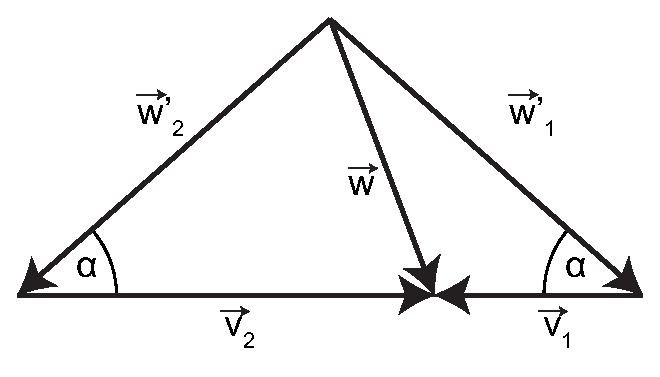
\includegraphics[width=0.4\textwidth]{2013-v3g-03-jalgrattur}\\
\end{center}
From the cosine formula:
$$
\begin{cases}
|\vec w|^2 = |\vec w'_1|^2 + |\vec v_1|^2  - 2  |\vec w'_2|  |\vec v_1|\cos \alpha \\
|\vec w|^2 = |\vec w'_2|^2 + |\vec v_2|^2  - 2  |\vec w'_2|  |\vec v_2|\cos \alpha.
\end{cases}
$$
Knowing that $ |\vec v_2|=2 |\vec v_1|$ and $ |\vec w'_1|=2 |\vec w'_2|$ we can multiply the first equation by two and subtract it from the second equation.
$$|\vec w|^2 = |\vec w'_1|^2 - 2|\vec v_1|^2. $$
This means that the actual speed of the wind is:
$$|\vec w|=\sqrt{|\vec w'_1|^2-2|\vec v_1|^2} \approx \SI{14}{km \per h}.$$
\fi
}